\documentclass[a4paper, landscape]{article}
\usepackage[utf8]{inputenc}
\usepackage{geometry}
\usepackage{fancyhdr}

\usepackage{graphicx}
\usepackage{tabularx}

\usepackage{amsmath}
\usepackage{amssymb}
\usepackage{amsthm}

\usepackage{multirow}
\usepackage{multicol}

\usepackage{enumitem}
\usepackage{array}
\usepackage{tikz}
\usepackage{color}

% https://www.micron.com/-/media/client/global/documents/products/technical-note/nand-flash/tn2942_nand_wear_leveling.pdf

% common variables
\def\name{Zusammenfassung Rechnersysteme}
\def\pages{2}

% custom settings
\geometry{top=2cm,bottom=2cm,left=1cm,right=1cm,landscape}

% common header and footer 
\pagestyle{fancy}
\fancyhf{}
\fancyhead[L]{\name}
\fancyhead[R]{Seite \thepage\hspace{1mm}von\hspace{1mm}\pages}
% \fancyfoot[C]{}

% common lenghts
\setlist{nosep}                 %Kein List Seperator
\setlength{\parindent} {0em}    %Kein Indent
\setlength{\columnseprule}{0.3pt}
\setlength{\topskip}{10pt}

% custom enviroments
\newenvironment{example}{
    \par\vspace{\abovedisplayskip}\noindent\textbf{Beispiel:}\par
}{\par\vspace{\belowdisplayskip}}
\newenvironment{important}{
    \par\vspace{\abovedisplayskip}\noindent\textbf{Wichtig:}\par
}{\par\vspace{\belowdisplayskip}}
\newenvironment{conditions}{
    \par\vspace{\abovedisplayskip}\noindent
    \tabularx{\columnwidth}{>{$}l<{$} @{${}={}$} >{\raggedright\arraybackslash}X}
}{\endtabularx\par\vspace{\belowdisplayskip}}

% custom commands
\newcommand*\circlenummber[1]{\tikz[baseline=(char.base)]{\node[shape=circle,draw,inner sep=0.1ex] (char) {#1};}}
\newcommand*\spaceline{\par\vspace{\belowdisplayskip}}

\title{\name}
\author{Louis Seubert}

\begin{document}
    \begin{multicols}{3}
        
        %         \begin{description}
        %             \item [RISC] (Reduced Instruction Set Computing)
        %             \item [CISC] (Complex Instruction Set Computing)
        %         \end{description}
        
        \section{Größen und Einheiten}
        
        \subsection{Datenmenge}
        \begin{center}
            \begin{tabular}{|c|c|c|c|c|c|c|}
                \hline \rule{0pt}{3ex} & \multicolumn{6}{c|}{Dezimalpräfix $\longrightarrow$}\\
                \hline \rule{0pt}{3ex}
                \multirow{6}{*}{\rotatebox[origin=center]{90}{$\longleftarrow$ Binärpräfix}} && \textbf{B} & \textbf{kB} & \textbf{MB} & \textbf{GB} & \textbf{TB} \\
                \cline{2-7}\rule{0pt}{3ex} & \textbf{B} & 1 & $10^{3}$ & $10^{6}$ & $10^{9}$ & $10^{12}$ \\
                \cline{2-7}\rule{0pt}{3ex} & \textbf{KiB} & $2^{10}$ & 1 & $10^{3}$ & $10^{6}$ & $10^{9}$ \\
                \cline{2-7}\rule{0pt}{3ex} & \textbf{MiB} & $2^{20}$ & $2^{10}$ & 1 & $10^{3}$ & $10^{6}$ \\
                \cline{2-7}\rule{0pt}{3ex} & \textbf{GiB} & $2^{30}$ & $2^{20}$ & $2^{10}$ & 1 & $10^{3}$ \\
                \cline{2-7}\rule{0pt}{3ex} & \textbf{TiB} & $2^{40}$ & $2^{30}$ & $2^{20}$ & $2^{10}$ & 1 \\
                \hline
            \end{tabular}
        \end{center}
        
        \subsection{Zeit}
        \[
        1\text{s} = 10^3\text{ms} = 10^9\text{ns}
        \]
        
        \section{Leistungsbewertung}
        \begin{important}
            MIPS-Vergleiche ergeben lediglich Sinn inerhalb der gleichen ISA (Instruction Set Architecture).
        \end{important}
        \[
        \text{MIPS} = \cfrac{10^3}{\text{Instruktionszeit in }ns}
        \]
        
        \subsection{Amdahls Gesetz}
        \begin{conditions}
            $G$ & Gesamtbeschleunigung \\
            $P$ & Anteil der Zeit, in dem die Verbesserung benutzt wird \\
            $(1 - P)$ & Anteil der Zeit, in dem die Verbesserung \textbf{nicht} benutzt wird \\
            $S$ & Beschleunigung welche Auftritt, wenn die Verbesserung benutzt wird \\
        \end{conditions}
        \begin{eqnarray}
            G &=& \cfrac{1}{(1 - P) + \cfrac{P}{S}}     \nonumber   \\
            S &=& \cfrac{G \cdot P}{1 - G + G \cdot P}  \nonumber   \\
            P &=& \cfrac{G \cdot S - S}{G \cdot S - G}  \nonumber
        \end{eqnarray}
        
        \section{Paritätsprüfung}
        
        \subsection{Paritätsbit}
        
        \subsection{Zyklische Redundanzprüfung}
        
        \section{Hamming-Code}
        
        \subsection{Anzahl der Prüf- und Datenbits}
        Für ein Wort der länge $n$ mit $m$ Datenbits benötigt man $r$ Prüfbits um einen 1-Bit-Fehler pro Wort zu korrigiren.
        Daraus ergibt sich folgende Ungleichung:
        \begin{eqnarray}
            2^r &=& m + r + 1       \nonumber \quad\text{für \textbf{perfekten} Hamming-Code}  \\
            2^r &\geq& m + r + 1    \nonumber
        \end{eqnarray}
        Ein perfekter Hamming-Code hat die Worllänge $2^r-1$.
        
        \subsection{Hamming-Abstand}
        Der Hamming-Abstand gibt die Anzahl der Bits zwischen zwei beliebige Wörtern aus dem Code.
        \begin{example}
            Die zwei Wörter $\texttt{1100100100}_2$ und $\texttt{1001100011}_2$ haben den Hamming-Abstand $h = 5$.
        \end{example}
        
        \subsubsection*{Hamming-Abstand eines Codes}
        Der Hamming-Abstand eines Codes ist die kleinstmögliche Anzahl an Bits, die man verändern muss um ein neues gültiges Wort aus dem vorliegenden Code zu bekommen.
        \begin{example}
            Da der kleinste Abstand 1 ist, ist der Hamming-Abstand des Codes ebenfalls 1.
            \par\centering
            \begin{minipage}{.35\linewidth}
                \begin{align}
                    x = \texttt{00110}  \nonumber   \\
                    y = \texttt{00101}  \nonumber   \\
                    z = \texttt{01110}  \nonumber
                \end{align}
            \end{minipage}
            \begin{minipage}{.35\linewidth}
                \begin{eqnarray}
                    h_{xy} &=& 2    \nonumber   \\
                    h_{xz} &=& 1    \nonumber   \\
                    h_{yz} &=& 3    \nonumber
                \end{eqnarray}
            \end{minipage}
        \end{example}
        
        \subsection{Fehlererkennung}
        Um $d$ Bitfehler zu erkennen, braucht man den Hamming-Abstand $h$:
        \begin{eqnarray}
            h &=& d + 1 \nonumber \\
            d &=& h - 1 \nonumber
        \end{eqnarray}
        
        \subsection{Fehlerkorrektur}
        Um $d$ Bitfehler zu korrigiren, braucht man den Hamming-Abstand $h$:
        \begin{eqnarray}
            h &=& 2d + 1 \nonumber \\
            d &=& \lfloor \cfrac{h - 1}{2} \rfloor \nonumber
        \end{eqnarray}
        
        \subsection{Bündelfehlerkorrektur}
        Um mehrere aufeinanderfolgende Bitfehler zu korrigiren ordnet man die $k$ mit Hamming codierten Wörter der Länge $n$ in einer $k \cdot n$ Matrix an.
        \emph{Dabei ist zu beachten das nun zuerst die erste Spalte der Matrix übertragen bzw. gespeichert wird.} \par
        Smit kann man einen \textbf{maximal} einen Bündelfehler der Länge $k$ Bits korrigiren, dabei ist bei $k$ aufeinanderfolgenden fehlerhaften Bits maximal 1 Bit pro Wort fehlerhaft.
        \begin{example}
         \begin{center}
            \begingroup\setlength\tabcolsep{2pt}
            \begin{tabular}{c|ccccccc|>{\bfseries}c>{\bfseries}cc>{\bfseries}cccc>{\bfseries}cccc}
                & \multicolumn{7}{c|}{ASCII} & \multicolumn{11}{c}{Codewort} \\
                \hline
                H & 1 & 0 & 0 & 1 & 0 & 0 & 0 & \circlenummber{0} & \circlenummber{0} & 1 & \circlenummber{1} & 0 & 0 & 1 & \circlenummber{0} & 0 & 0 & 0 \\
                a & 1 & 1 & 0 & 0 & 0 & 0 & 1 & \circlenummber{1} & \circlenummber{0} & 1 & \circlenummber{1} & 1 & 0 & 0 & \circlenummber{1} & 0 & 0 & 1 \\
                m & 1 & 1 & 0 & 1 & 1 & 0 & 1 & \circlenummber{1} & \circlenummber{1} & 1 & \circlenummber{0} & 1 & 0 & 1 & \circlenummber{0} & 1 & 0 & 0 \\
                m & 1 & 1 & 0 & 1 & 1 & 0 & 1 & \circlenummber{1} & \circlenummber{1} & 1 & \circlenummber{0} & 1 & 0 & 1 & \circlenummber{0} & 1 & 0 & 0 \\
                i & 1 & 1 & 0 & 1 & 0 & 0 & 1 & \circlenummber{0} & \circlenummber{1} & 1 & \circlenummber{0} & 1 & 0 & 1 & \circlenummber{1} & 0 & 0 & 1 \\
                n & 1 & 1 & 0 & 1 & 1 & 1 & 0 & \circlenummber{0} & \circlenummber{1} & 1 & \circlenummber{0} & 1 & 0 & 1 & \circlenummber{0} & 1 & 1 & 0 \\
                g & 1 & 1 & 0 & 0 & 1 & 1 & 1 & \circlenummber{0} & \circlenummber{1} & 1 & \circlenummber{1} & 1 & 0 & 0 & \circlenummber{1} & 1 & 1 & 1
            \end{tabular}
            \end{center}
            \endgroup
            Die übertragenen Bits lauten:\par
            \texttt{0111000 0011111 1111111 1100001 0111111 0000000}\par
            \texttt{1011110 0100101 0011011 0000011 0100101}
        \end{example}

        
        \subsection{Hamming-Algorithmus}
        
        \subsubsection*{Paritäts-Kontrollbits}
        Paritäts-Kontrollbits $p$ an Zweierpotenz Positionen
        \begin{itemize}
            \item Paritätsbit $p_{1}$ prüft 1, 3, 5, 7, 9, 11, 13, 15, 17, 19, 21
            \item Paritätsbit $p_{2}$ prüft 2, 3, 6, 7, 10, 11, 14, 15, 18, 19
            \item Paritätsbit $p_{4}$ prüft 4, 5, 6, 7, 12, 13, 14, 15, 20, 21
            \item Paritätsbit $p_{8}$ prüft 8, 9, 10, 11, 12, 13, 14, 15
            \item Paritätsbit $p_{16}$ prüft 16, 17, 18, 19, 20, 21
        \end{itemize}
        
        \begin{example}
         \begingroup\setlength\tabcolsep{1.9pt}\scriptsize
            \begin{tabular}{cccccccccccccccccccccc}
             Position   & \textbf{1} & \textbf{2} & 3 & \textbf{4} & 5 & 6 & 7 & \textbf{8} & 9 & 10 & 11 & 12 & 13 & 14 & 15 & \textbf{16} & 17 & 18 & 19 & 20 & 21 \\
             \hline
             Wert       & \textbf{?} & \textbf{?} & 1 & \textbf{?} & 1 & 1 & 1 & \textbf{?} & 0 & 0 & 0 & 0 & 1 & 0 & 1 & \textbf{?} & 0 & 1 & 1 & 1 & 0 \\
             + Parität  & \textbf{0} & \textbf{0} & 1 & \textbf{0} & 1 & 1 & 1 & \textbf{0} & 0 & 0 & 0 & 0 & 1 & 0 & 1 & \textbf{1} & 0 & 1 & 1 & 1 & 0 \\
            \end{tabular}
         \endgroup
        \end{example}

        \section{Fehlertoleranz}
        
        \subsection{N-Modulare-Redundanz}
        \paragraph{2MR} W
        
        \paragraph{3MR} W
        
        \paragraph{4MR} W
        
        \paragraph{5MR} W
        
        \section{Speicher}
        
        \subsection{HDD}
        
        \subsubsection{Definitionen}
        \textbf{Spur} ist ein Kreis auf der die Sektoren nacheinander angeordnet sind. Diese Spuren liegen konzentrisch auf der Festplatte.
        \spaceline
        \textbf{Sektor} ist ein Teilstück einer Spur welches eine feste Länge besitzt, meist 512 bzw. 4096 Bits lang.
        \spaceline
        \textbf{Zylinder} ist eine vertikale Zusammenfassung übereinander liegender Spuren.
        \spaceline
        Durch diese Unterteilung kann man jeden Datenblock durch seine Kopf-, Zylider- und Sektorennummer identifiziren. 
        Dieser Identifizierungsnummer stehe in der \textbf{Präambel} (PRE) des Sektors. 
        Gefolgt kommen die Nutzdaten und eine \textbf{Fehlererkennung/-korrektur} (ECC)
        
        \begin{center}
         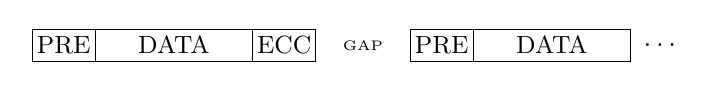
\begin{tikzpicture}[scale=0.40]
             \draw (00,00) rectangle (02,01) node[pos=0.5] {\small{PRE}};
             \draw (02,00) rectangle (07,01) node[pos=0.5] {\small{DATA}};
             \draw (07,00) rectangle (09,01) node[pos=0.5] {\small{ECC}};
             \path (09,00) rectangle (12,01) node[pos=0.5] {\tiny{GAP}};
             \draw (12,00) rectangle (14,01) node[pos=0.5] {\small{PRE}};
             \draw (14,00) rectangle (19,01) node[pos=0.5] {\small{DATA}};
             \path (20,0.5) node {\ldots};
         \end{tikzpicture}
        \end{center}

        \subsubsection{Datenübertragungszeit}
        \begin{conditions}
            $$B_{\text{file}}$$ & Größe der Datei\\
            $$B_{\text{sector}}$$ & Größe eines Sektors \\
            $$N_{\text{surface}}$$ & Anzahl der Oberflächen der Festplatte \\
            $$N_{\text{sector}}$$ & Anzahl der Sektoren pro Spur \\
            $$T_{s}$$ & Zeit für die Positionierung zum Start des Vorgangs \\
            $$T_{r}$$ & Zeit für die Positionierung zwischen benachbarten Spuren \\
            $$V_{\text{d}}$$ & Rotationsgeschwindigkeit [rps] \\
            $$T_{\text{sr}}$$ & Zeit für \textbf{eine} Umdrehung \\
            $$T_{\text{latency}}$$ & Zeit der Rotationsverzögerung \\
            \\
            $S$ & Anzahl der benötigten Spuren \\
            $$T_{s}$$ & Zeit für die Positionierung zum Start des Vorgangs \\
            $$T_{r}$$ & Mittlere Latenz Zeit bis Präambel gelesen wird \\
            $$T_{t}$$ & Zeit für den Datentransfer \\
            $$n$$ & Umdrehungen pro Minute
        \end{conditions}
        
        \[
        S = \cfrac{\text{Datei}_\text{Größe}}{\text{Oberflächen}_\text{Anzahl} \cdot \text{Sektoren}_\text{Anzahl} \cdot \text{Sektor}_\text{Größe}}
        \]
        
        \[
        T_{t} = \cfrac{60 \cdot 1000}{n}
        \]
        
        \[
        T_{r} = \cfrac{T_{w}}{2}
        \]


        
        \[
        T = T_{s} + T_{r} + T_{t}
        \]

        
        \[
        T_{\text{average}} = T_{\text{first track}} + T_{\text{extra track}}
        \]
        
        \[
        T_{\text{latency}} = \cfrac{1}{2} \cdot T_{r}
        \]
        
        \[
        T_{\text{first track}} = T_{s} + T_{\text{latency}} + T_{sr}
        \]
        
        \[
        T_{\text{extra track}} = ( T_{r} + T_{\text{latency}} + T_{sr} ) \cdot ( N_{\text{tracks}} - 1 )
        \]




         
%         \begin{align}
%             T_{average} &=& \nonumber\\
%             & ( T_{ps} + T_{\text{latency}} + T_{sr} ) \nonumber\\
%             & \quad + [( T_{pn} + T_{\text{latency}} + T_{sr} ) \cdot ( N_{\text{tracks}} - 1 )] \nonumber
%         \end{align}
         
        
        \subsection{SSD}
        \begin{conditions}
            $$C$$ & Lösch/Schreib-Zyklen pro Speicherzelle                                  \\
            $$T_{L}$$ & Lebensdauer                                                         \\
            $$B_{G}$$ & Gesamtanzahl der Blöcke                                             \\
            $$B_{T}$$ & Anzahl der Blöcke welche pro Zeiteinheit geschrieben werden         \\
            $$P_{D}$$ & Prozentanteil der dynamischen Daten                                 \\
            $$P_{S}$$ & Prozentanteil der reservierten Blöcke für das Bad Block Management
        \end{conditions}
        
        \[
        B_{G} = \cfrac{\text{Kapazität}}{\text{Blockgröße}} \cdot ( 1 - P_{S} )
        \]

        \subsubsection*{Static Wear Levelling}
        \[
            T_{L} = \cfrac{C \cdot B_{G}}{B_{T}}
        \]
        
        \subsubsection*{Dynamic Wear Levelling}
        \[
            T_{L} = \cfrac{C \cdot ( B_{G} \cdot P_{D} )}{B_{T}}
        \]

        
    \end{multicols}
\end{document}
